% !TEX root = ../paper.tex
\section{Implementation Details and Challenges}\label{sec:implementation}

\subsection{``Everything is a Set''}\label{sec:everything-is-a-set}
The predominantly relational nature of Forge introduces a point of friction between our translation from Forge to Lean. In Forge, every expression is implicitly a relation or a set (set when that expression has arity-1\footnote{The notation we use is that a \texttt{Set α}, which has equivalent type \texttt{α → Prop}, has arity-1, and so on. This is the arity convention in Forge and aligns with Lean's definitions of relations.}). Even when we know that an expression is a relation or set with cardinality 1 (for example, it could be introduced as a binder from a quantification), they are used as if they were a singleton set in Forge expressions that expect a set as an operand. Under the hood, all expressions in Forge are treated as a set (or multi-arity relation). 

This everything-is-a-set approach of Forge allows the following expression (within the existential quantifier), translated ``there is some \texttt{Student} who is their own friend'': 

\vspace{0.5em}
\noindent\begin{minipage}{0.5\textwidth}
\begin{forge*}
sig Student {
  friends : set Student
}
pred ownFriend {
  some s: Student |
    s in s.friends
}
\end{forge*}
\end{minipage}%
\begin{minipage}{0.5\textwidth}
\begin{lean*}
opaque Student : Type
opaque friends : Student → Student → Prop

def ownFriend := 
  ∃ s : Student, 
    friends s s
?\phantom{}?
\end{lean*}
\end{minipage}
\vspace{0.5em}\newline
Note that \texttt{s} is a `singleton', but it is used as if it were an honest-to-goodness set in the join operation (\texttt{s.friends}) and the inclusion operation (\texttt{s in }...). We can concisely translate into a statement in Lean of the likes of ``$\exists s$ such that on the \texttt{friends} relation, $(s,s)\in \texttt{friends}$.'' Note that because \texttt{s} is a singleton---that is, no set with more than one element could be bound to \texttt{s} as a result of our existential quantifier---we were able to translate the join in $\texttt{s} \bowtie \texttt{friends}$ as the partial application to our relation \texttt{friends s}, and the \texttt{in} keyword became set membership $\texttt{s}\in \texttt{s} \bowtie \texttt{friends}$ which was just \texttt{(friends s) s}. 

Consider an alternative when we relax the requirement that \texttt{s} ought to be a singleton in the Forge source: 

\vspace{0.5em}
\noindent\begin{minipage}{0.5\textwidth}
\begin{forge*}
pred ownFriend[t: Student] {
  let s = t.friends |
    s in s.friends
}
\end{forge*}
\end{minipage}%
\begin{minipage}{0.5\textwidth}
\begin{lean*}
def ownFriend (t : Student) := 
  let s := friends t, 
    friends s s -- Type error!
?\phantom{}?
\end{lean*}
\end{minipage}
\vspace{0.5em}\newline
Which is loosely ``for a \texttt{Student} \texttt{t}, the set of \texttt{t}'s friends is a subset of the set of all \emph{their} friends.'' Here, \texttt{s} in Forge is bound to a set of \texttt{t}'s friends. Had we translated this in the same way, \texttt{s} would be typed \texttt{Student → Prop} (or equivalently, a \texttt{Set Student}), and \texttt{friends s s} raise a type error. 

We instead have to resolve the join $\texttt{s} \bowtie \texttt{friends}$ without our shortcut above of partially applying \texttt{s} to \texttt{friends}: 

\vspace{0.5em}
\noindent\begin{minipage}{0.3\textwidth}
\begin{forge*}
s.friends
\end{forge*}
\end{minipage}%
\begin{minipage}{0.7\textwidth}
\begin{lean*}
λ x₂ ↦ ∃ x₁ : Student, s x₁ ∧ friends x₁ x₂
\end{lean*}
\end{minipage}
\vspace{0.5em}\newline
which is immediately more cumbersome than our earlier solution. 

The same applies when we now try to implement the inclusion \texttt{in} operator: 

\vspace{0.5em}
\noindent\begin{minipage}{0.3\textwidth}
\begin{forge*}
s in s.friends
\end{forge*}
\end{minipage}%
\begin{minipage}{0.7\textwidth}
\begin{lean*}
Set.Subset s (λ x₂ ↦ ∃ x₁ : Student, s x₁ ∧ friends x₁ x₂)
\end{lean*}
\end{minipage}
\vspace{0.5em}\newline
which becomes a subset operator\footnote{Under the hood, \texttt{Set.Subset s₁ s₂} is defined as \texttt{∀ a, a ∈ s₁ → a ∈ s₂}.} instead of set membership. 

This example describes a fundamental incompatibility between Forge and Lean that we need to resolve. Forge is indifferent between whether an expression is a singleton or a relation/set and treats the two indiscriminately. This approach of treating everything as a set allows operations like relational join and `in' to work across all scenarios alike. 

However, Lean tends to prefer expressions that are not sets (that is, honest-to-goodness singletons). In the cases above, this allows for relational join to be a partial application, and `in' to be set membership. For the majority of use cases, this singleton-friendly translation suffices. When we are dealing with sets, set operators such as join and `in' (which is now the subset operator) become more convoluted as demonstrated above. Additionally, while joining a singleton and a relation via the partial application solution applies to relations of varying arities, a join expression between two arbitrary relations takes in different types, and hence implementations, depending on the respective arities and types of the arguments. 

This means that we shouldn't take the same approach as Forge of treating everything as a set and performing the most generic set operation possible on them. Where possible, we ought to keep elements as elements and not cast them into singleton sets, since cutting this corner in translation necessarily comes at the cost that the output of the translation is more complicated. 

The outline of our solution is to consistently emit only the simplest (and most type-tailored) translation possible, leveraging the fact that we know at the time of translation all types of inputs into an operator. We implement this through Lean's type class system, where a set of methods can be implemented across different types and dispatched according to the type of its arguments. For every pair of types for which a method might be different (in other words, overloaded), we can write an instance of that type class implementing its functionality. 

For example, the following is an excerpt\footnote{There is an instance for every pair of arities and types that could be passed into a join, hence there are many more instances than shown here. However, these implementation details are obscured to the end-user since the join function \texttt{HJoin.join} will only resolve to a single instance.} of our implementation of relational join\footnote{We use ``$\bowtie$'' to denote the relational join operator. If $x: A \to B$ is a relation and $y: B \to C$ is a relation, then $x\bowtie y$ produces the relation $A\to C$ merged on common values in the rightmost ($B$) column of $x$ and the leftmost ($B$) column of $y$. $x$ and $y$ can be of arbitrary arity, so long as their leftmost and rightmost columns respectively match. That is, on $n$-ary relation $A$ and $m$-ary relation $B$, 
\[A \bowtie B := \{(a_n, \dots, a_{n-1}, b_2, \dots, b_m) \mid \exists x, (a_1, \dots, a_{n-1}, x)\in A \land (x, b_2, \dots, b_m)\in B\}.\]
} as a type class \texttt{HJoin} (`has join'), following our implementations of join from the examples demonstrated above: 

\begin{leanimpl*}
class HJoin (α : Type) (β : Type) (γ : outParam Type) :=
  (join : α → β → γ)

-- Join singleton with arity-2 relation
@[reducible, simp] instance {α β : Type} : HJoin (α) (α → β → Prop) (β → Prop) where
  join := fun a g ↦ g a

-- Join set with arity-2 relation
@[reducible, simp] instance {α β : Type} : HJoin (α → Prop) (α → β → Prop) (β → Prop) where
  join := fun l r b ↦ ∃ a : α, l a ∧ r a b
\end{leanimpl*}

Then, when translating $\texttt{a}\bowtie \texttt{b}$, we can indiscriminately produce \texttt{HJoin.join a b} and have Lean synthesize which particular implementation to apply based on the types of \texttt{a} and \texttt{b}. This allows us to have the most specific translation of an expression depending on the types of operands. The \texttt{simp} attribute on the instances allows the Lean simplifier (calling the \texttt{simp} tactic) to consult this as an unfoldable definition at proof-time and we are left with the native meaning.

For many operators on expressions (see \cref{sec:join-cross-subset} below), their implementations in Lean are overloaded to accommodate the fact that Lean prefers elements when they are elements and sets only when necessary, contrasted to Forge's `everything-is-a-set' approach. This allows us to produce semantically equivalent translations that are more simplified when possible leveraging Lean's type class system that can determine types of operands at the time of translation. 

\subsection{Relational Joins, Cross, Inclusion, Equality}\label{sec:join-cross-subset}

We need to take special care when implementing expression operators in Lean whenever one of these conditions is true: 
\begin{enumerate}[(1)]
  \item There is no direct out-of-the-box translation for a Forge operation within Lean, or
  \item there are several implementations of a Forge operation in Lean, depending on the types of the operands given, and where the most generic might not necessarily be the simplest. 
\end{enumerate}
We discuss (2) extensively in \cref{sec:everything-is-a-set}, and introduce using Lean's type class system to implement varying translations of a method depending on the input types. There are several other Forge operations that require this treatment: membership, join (introduced above), cross, and equality. 

The specific operators that we needed to take special care translating, the different types that they permit, and their translations in Lean are detailed below in \cref{tab:forge-operators}. 

When we do specify special Forge operators, we additionally specify custom infix operators for our operations to pretty-print in the Lean infoview window (see \cref{fig:mutex-proof} for an example): 
\begin{leanimpl*}
  infix:50 !\texttt{\textquotedbl }$\bowtie$\texttt{ \textquotedbl}! => HJoin.join
\end{leanimpl*}
so translated statements look like $\texttt{a}\bowtie\texttt{b}$ instead of \texttt{Forge.HJoin.join a b}. 

% Some shifting happened here:
\newpage
\begin{table}[h!]
\renewcommand{\arraystretch}{1.2}
\centering
\caption{Forge binary operators and corresponding implementations based on operand types.\newline}
\label{tab:forge-operators}
\begin{tabular}{@{}l >{\columncolor{forgelistingcolor}}l >{\columncolor{leanlistingcolor}}l@{}}
\hline
\textbf{Forge Operator} &
  \cellcolor{white}\begin{tabular}[c]{@{}l@{}}\textbf{Possible Types}\\[-0.9em] \tiny{(singletons lowercase, sets uppercase)}\end{tabular} &
  \cellcolor{white}\textbf{Lean Implementation} \\ \hline
Membership: \texttt{a in b}         & \texttt{a in b} & \texttt{a = b}                 \\
                                    & \texttt{a in B} & \texttt{a ∈ B}                 \\
                                    & \texttt{A in b} & \texttt{A = Set.singleton b}   \\
                                    & \texttt{A in B} & \texttt{A ⊆ B}                 \\
Equality: \texttt{a = b}            & \texttt{a = b}  & \texttt{a = b}                 \\
  &
  \texttt{a = B} or \texttt{A = b} &
  \texttt{Set.singleton a = B}, or vice versa. \\
                                    & \texttt{A = B}  & \texttt{A = B}                 \\
Join: \texttt{a.b} or \texttt{b[a]} & \texttt{a.B}    & \texttt{B a}                   \\
                                    & \texttt{A.B}    & \textit{Varies, see \cref{sec:everything-is-a-set}.} \\
Cross: \texttt{a->b}                & \texttt{a->b}   & \texttt{(a, b)}                \\
  &
  \texttt{a->B} or \texttt{A->b} &
  \textit{Varies}, like \texttt{λ a f a' b ↦ a = a' ∧ f b} \\
                                    & \texttt{A->B}   & \texttt{λ f g a b ↦ f a ∧ g b} \\ \hline
\end{tabular}
\end{table}

\newpage
\subsection{Boundedness of Forge Sigs}\label{sec:finiteness}
Recall as summarized in \cref{sec:forge-model} that Forge Sigs get (most naturally) translated to Lean Types. However, we need to be cautious about using this as a drop-in replacement for the concept of sigs. While we don't have soundness and completeness guarantees, we ought to feel confident that our translation preserves the semantics of Forge faithfully\footnote{See \cref{sec:future-work} for a discussion of formal guarantees.}. 

One semantic difference in translating Forge Sigs into Lean Types directly is that we lose all sig `bounded guarantees' that came with Forge. Since Forge compiles to a bounded SAT problem, it operates under the assumption that all sigs are finitely bounded. This means that we can rely on the assumption that sets of sigs are all finite sets. 

For example, we could write a specification of a graph with an injective \texttt{next} function and the existence of a root node that is not in the image of \texttt{next}. 
\begin{forge*}
sig Node {
  next: one Node
}

pred injective {
  all a, b : Node | 
    a.next = b.next => a = b
}

pred someRoot {
  some r : Node | 
    no next.r
}
\end{forge*}
For any number of \texttt{Node} sigs we initialize Forge with (that is, for any bandwidth), Forge will be able to tell us that \texttt{¬(injective ∧ someRoot)} is theorem (that is, no such relation can exist). 

Yet, in the Lean formulation of this specification, we realize that \texttt{injective ∧ someRoot} could be true! If we tried to prove the same in Lean, we realize that it isn't actually possible to prove the injectivity of our next relation. In fact, if we conjured our type \texttt{Node} with the same structure as $\NN$, we would have a perfectly valid \texttt{next} function (\texttt{succ}) that is injective and $0$ has no predecessor. 

The disparity between the Forge and Lean models is that while Forge models are bounded, Lean makes no assumption about the size of models or types and requires us to make explicit statements of the finiteness of types. For the semantics of Lean to match that of Forge being finite, we need guarantees that any types from Lean sigs are finite types. 

Our solution is to include additional local instance axioms for every opaque sig that is translated from Forge and introduced to our Lean environment. In this case: 
\begin{lean*}
@[instance] axiom inhabited_node : Inhabited Node
@[instance] axiom fintype_node : Fintype Node
\end{lean*}
which gives us guarantees that \texttt{Node} is both inhabited\footnote{We are required to do this to, say, create functions and subtypes on these types. See \cref{sec:sigs} for how we handle the \texttt{abstract} quantifier.} and contains a finite number of elements within the type. To illustrate, our proof of \texttt{injective ∧ someRoot} would utilize the pigeonhole principle and appeal to the fact that \texttt{Node} is finitely inhabited, and that for a root node to exist there must be a node that has 2 predecessors. 

We discuss further in \cref{sec:integers} how these instances enable us to perform integer and cardinality operations on sigs and translated Forge expressions. 


\subsection{Sig Inheritance and Quantifiers}\label{sec:sigs}
\subsubsection{Inheritance}
Many signatures in Forge have complex inheritance structures \cite{jackson2012software} that cannot be expressed in Lean using a na\"ive translation. Recall that conventionally, we would translate a signature in Forge into a corresponding opaque type in Lean as follows (see \cref{sec:forge-model}):

\vspace{0.5em}
\noindent\begin{minipage}{0.5\textwidth}
\begin{forge*}sig Student {}\end{forge*}
\end{minipage}%
\begin{minipage}{0.5\textwidth}
\begin{lean*}opaque Student : Type\end{lean*}
\end{minipage}
\vspace{0.5em}

However, how then would we represent another sig like \texttt{Undergrad} which inherits from a \texttt{Student} sig? In Forge, we can use the \texttt{extends} keyword to denote that \texttt{Undergrad} inherits fields from \texttt{Student}: 
% \forge{}
\begin{forge*}
sig Undergrad extends Student {}
\end{forge*}

For \texttt{Undergrad} to \emph{extend} \texttt{Student}, every field accessible to \texttt{Student} must also be available to \texttt{Undergrad}, and any expression of the \texttt{Undergrad} type should be interchangeable as expressions of type \texttt{Student}. 

As we did before, we could try to define the corresponding type in the same way, without any regard to the fact that it inherits from such a parent sig: 
\begin{lean*}
opaque Undergrad : Type
\end{lean*}
However, Lean does not know that all \texttt{Undergrad}s are also \texttt{Student}s, and since fields are typed to the sig that they are a part of in Lean\footnote{For sig \texttt{A} to have a field \texttt{f : set A} is for the field \texttt{f} to have type \texttt{A → A → Prop}.}, any access into a field that belongs to the \texttt{Undergrad} sig inherited because it was part of the \texttt{Student} sig would fail. Consider the following Forge program and the wishfully translated Lean equivalent:

\vspace{0.5em}
\noindent\begin{minipage}{0.5\textwidth}
\begin{forge}
sig Class {}
sig Student {
  registration : set Class
}
sig Undergrad extends Student {}

fun ugradsIn[c : Class] : Undergrad {
  all u : Undergrad |
    c in u.registration
}
\end{forge}
\end{minipage}%
\begin{minipage}{0.5\textwidth}
\begin{lean*}
opaque Class : Type
opaque Student : Type
opaque registration : Student → Class → Prop

opaque Undergrad : Type

def ugradsIn (c : Class) : Set Undergrad :=
  ∀ u : Undergrad, 
    registration u c -- Type error!
?\phantom{}?
\end{lean*}
\end{minipage}
\vspace{0.5em}

Such a Lean translation would raise a type error at line 9 above as \texttt{registration} expects an object of the \texttt{Student} type for its first input but was given a \texttt{Undergrad} type instead. In the case of Forge, Forge is aware that all descendents of a particular sig can be used interchangeably when an expression of that sig is expected. We need to find a (clever) way to encode within Lean that in fact, \texttt{Undergrad} is a child sig of \texttt{Student} and all \texttt{Undergrad}s are \texttt{Student}s. As Lean is not `object-oriented' in the way that Forge is, there is no directly equivalent concept of a type that inherits from another type in Lean natively. 

This task has its subtleties and at the same time, we will need to keep usability in mind for an end-user who wishes to prove facts about their model. One direct solution motivated by our type error might be to introduce a coercion instance from \texttt{Undergrad}s to \texttt{Grad}s which immediately fixes our problem:
\begin{lean*}@[instance] axiom coe_undergrad_student : Coe Undergrad Student\end{lean*}
The code snippet above would type check, and we would instantly be able to refer to the child sig in place of its parent sig. However, if we wish to query in a proof whether a \texttt{Student} object is an \texttt{Undergrad} object as well via a predicate like \texttt{IsUndergrad}\footnote{This is the \texttt{Undergrad} membership predicate on \texttt{Student}s, which we'll likely need to do to prove anything about objects within this inheritance relation.}, this becomes burdensome and involved:
\begin{lean*}def IsUndergrad (s : Student) : Prop := ∃ x : Undergrad, x = s\end{lean*}
The existential which quantifies over all \texttt{Undergrad}s to check if they are equal to \texttt{s} is not very user-friendly and can become significantly involved, especially when we are utilizing inheritance liberally in a specific model. Furthermore, we have no straightforward solution given \texttt{(IsUndergrad u)} and \texttt{(u: Student)} to cast \texttt{u} back into an \texttt{Undergrad} type. 

Instead, we can consider switching the order we define the child type and child type predicate to the dual of the translation above. If instead we define our membership predicate \texttt{IsUndergrad} first:
\begin{lean*}opaque IsUndergrad : Student → Prop\end{lean*}
we can then use Lean's native subtyping to define our \texttt{Undergrad} type:
\begin{lean*}
@[reducible] def Undergrad : Type :=
  { s : Student // IsUndergrad s }
\end{lean*}
In this implementation, we also happen to get the \texttt{Undergrad} to \texttt{Student} coercion automatically as a property of subtyping.

\subsubsection{Abstract Sigs}

In addition, Forge introduces the concept of \emph{abstract} sigs \cite{jackson2012software}. If \texttt{Student} were an abstract sig, we might encounter \texttt{Undergrad} and \texttt{Grad} student as concrete subtypes of \texttt{abstract Student}, like:
\begin{forge*}
abstract sig Student {}
sig Undergrad extends Student {}
sig Grad extends Student {}
\end{forge*}
which is to say that every object instance of \texttt{Student} had ought to be either a \texttt{Undergrad} or \texttt{Grad}. Within our framework, this can be implemented in Lean as
\begin{lean*}
axiom abstract_student : ∀ s : Student, IsUndergrad s ∨ IsGrad s
\end{lean*}
provided both subtype instances for \texttt{Undergrad} and \texttt{Grad} have been generated correctly. 

To inform Lean that our subtypes are distinct and unique, for each pair of subtypes, we generate an axiom with the \texttt{simp} modifier that states each subclass is disjoint: 
\begin{lean*}
@[reducible,simp] axiom disjoint_Student_IsUndergrad_IsGrad : 
  ∀ s : Student, ¬ (IsUndergrad s ∧ IsGrad s)
\end{lean*}

\subsubsection{One Sigs}

If furthermore, \texttt{Undergrad} and \texttt{Grad} are \texttt{one} sigs without fields, they are not generated as subtypes but instead are generated as opaque elements of \texttt{Student}, with their membership predicates being defined as equality: 
\begin{lean*}
opaque Undergrad : Student
def IsUndergrad (s : Student) := (Undergrad = .)
\end{lean*}

For \texttt{one} sigs with fields, we still need the sig to be a type in Lean so we can construct the fields relating to that sig. In this case, we have defined a type class of \texttt{One} that contains the single element \texttt{One.one} and a proof that all elements of this type are equal to this element: 
\begin{leanimpl*}
class SigQuantifier.One (α : Type) :=
  one : α
  allEq : ∀ x : α, x = one
\end{leanimpl*}
and we also introduce a corresponding coercion from a \texttt{One α} to the single element of type \texttt{α}, which is discussed further in \cref{sec:type-coercions}.
\subsubsection{Processing Sigs}

Such an analysis and translation of inheritance requires a global processing of the Forge program in Lean, since every expression emitted by our elaborator ought to have well-defined types and terms (that is, cannot be waiting for a term to be defined). Since Forge fields can depend on any sig, we need to `lift' sigs to define first before all fields and predicates can be defined. Furthermore, sig quantifiers and inheritance structures require preprocessing all sigs to generate a topological sort of the inheritance structure before expressing any of their translations in Lean. Since Forge is not a `local' language and all sig declarations are lifted, this was not a problem for us before we entered Lean. As such, sigs can be specified in any order in Forge. 

For the remaining of sig quantifiers like \texttt{one} and \texttt{lone}, because of their complex interactions with inheritance (a \texttt{one} sig means that there is only one inhabited member of that sig that \emph{is not} any child sig, contrary to our intuition as to what a \texttt{one} or \texttt{lone} sig should be), our program prompts the user to write a customized axiom in Lean expressing their desired constraint. Note that this utilizes the seamless integration of Forge into Lean which makes such a solution of mixed execution possible. Anecdotally, \texttt{one} and \texttt{lone} sigs only apply to child sigs and the \texttt{abstract} quantification is only used on parent sigs (it doesn't make sense for a non-inherited sig to be \texttt{abstract}), so we expect that manual handling of sig quantifications to be an edge case. 


\subsection{Typing \& Type Coercions}\label{sec:type-coercions}
While Forge treats all expressions as sets (see \cref{sec:everything-is-a-set}), there can often be several ways to represent a set-like object in Lean. 

The most common representation of a set of type \texttt{α} is \texttt{α → Prop}, which can be thought of as the membership predicate representing that set. This is oftentimes useful since checking set membership of \texttt{x : α} on set \texttt{s : α → Prop} is just a functional application: \texttt{s x}. This is also the canonical representation of sets in Lean: a \texttt{Set α} is definitionally equal to \texttt{α → Prop}, and \texttt{a ∈ b} is definitionally equal to \texttt{b a}. These representations can, for the most part, be used interchangeably. 

\subsubsection{Singletons as Sets}

However, there are additional expressions that Forge sees as sets but Lean does not. An element \texttt{x : α} is a singleton set, which we discuss extensively in \cref{sec:everything-is-a-set}. When possible, we can use type classes to `tailor' an operation to whether an expression is a singleton or a true set; and the different implementations are detailed in \cref{sec:join-cross-subset}. 

However, we need an `escape plan' if no such tailored implementation exists. Hence, we include a coercion from all singletons to sets of singletons. At worst, we can treat individual elements as the set containing just them\footnote{The implementation of \texttt{coe} has type \texttt{α → α → Prop}, which we can implement point-free---and there is a desire for syntactically simpler translations which are easier to work with in the Lean environment.}: 
\begin{leanimpl*}
instance : Coe α (α → Prop) where
  coe := Eq
\end{leanimpl*}

\subsubsection{Sigs as Sets}

Additionally, a translated sig \texttt{(α : Type)} is expected to denote the set of all elements in that sig. For example:
\begin{forge}
pred isAFriend[s: Student] {
  s in Student.friends
}
\end{forge}
is the predicate that \texttt{s} is \emph{someone}'s friend, where the set of all friends is the join of $\texttt{Student} \bowtie \texttt{friends}$ (which is equivalent to the set comprehension expression \texttt{\{s: Student | some t: Student | s in t.friends\}}). Here, \texttt{Student} is being used to denote the \emph{type} of \texttt{s} on line 1 and the set corresponding to type \texttt{Student} on line 2. 

In our translation, we want to be able to use the type \texttt{Student} interchangeably in places that expect a set of type \texttt{Student} as the set of all \texttt{Student}s. Since we included our finiteness \texttt{Fintype} property as an instance when translating sigs (see \cref{sec:finiteness}), we can create a coercion that coerces a Lean \texttt{Type}, given that it is a finite type, into a set of that type using the definition of the \texttt{Fintype} typeclass. 
\begin{leanimpl*}
instance [f: Fintype α] : CoeDep Type (α : Type) (Set α) where
  coe := (f.elems : Set α)
\end{leanimpl*}

When a sig is quantified \texttt{one} (see \cref{sec:sigs}), we also have a corresponding coercion of that sig into the single value that inhabits it: 
\begin{leanimpl*}
@[reducible, simp] instance [o: SigQuantifier.One α] : CoeDep Type (α : Type) α where
  coe := o.one
\end{leanimpl*}

\subsubsection{Multi-arity Sets}

Furthermore, there are additionally more ways of representing multi-arity relations in Lean that aren't immediately interchangeable. Where \texttt{Set α} and \texttt{α → Prop} are definitionally the same type, \texttt{Set (α × β)} and \texttt{α → β → Prop} are not. For each arity, we need to make use of either \texttt{Function.curry} and \texttt{Function.uncurry}, or custom coercion functions, to interchange between the two, for example: 
\begin{leanimpl*}
instance : Coe (Set (α × β)) (α → β → Prop) where
  coe := Function.curry

instance : Coe (α → β → Prop) (Set (α × β)) where
  coe := Function.uncurry

instance : Coe (Set (α × β × γ)) (α → β → γ → Prop) where
  coe := fun s ↦ fun a b c ↦ (a, b, c) ∈ s

instance : Coe (α → β → γ → Prop) (Set (α × β × γ)) where
  coe := fun r ↦ {p : α × β × γ | r p.1 p.2.1 p.2.2}
\end{leanimpl*}
Future work will involve attempting to remove cross products and standardize all multi-arity sets, which are currently introduced by Forge cross products (see \cref{sec:join-cross-subset}). 

\subsubsection{Explicit Coercions}

The Lean elaborator, which is responsible for type unifications, is occasionally unable to find such coercions we have introduced due to having many possible paths of coercion. This is further exacerbated by the fact that our type might appear in an expression where we have encoded several implementations (like equality, see \cref{sec:join-cross-subset}). 

In situations such as these, we might encounter type errors even when coercions should have been taken, such as 
\begin{forge*}
pred raise[pre: State, p: Process, post: State] {
  pre.loc[p] = Uninterested
  post.loc[p] = Waiting
  post.flags = pre.flags + p -- Type error!
  all p2: Process | p2 != p => post.loc[p2] = pre.loc[p2]
}
\end{forge*}
which produces the following error\footnote{This example is taken from \cref{sec:mutex}.}:

\begin{center}
  \fbox{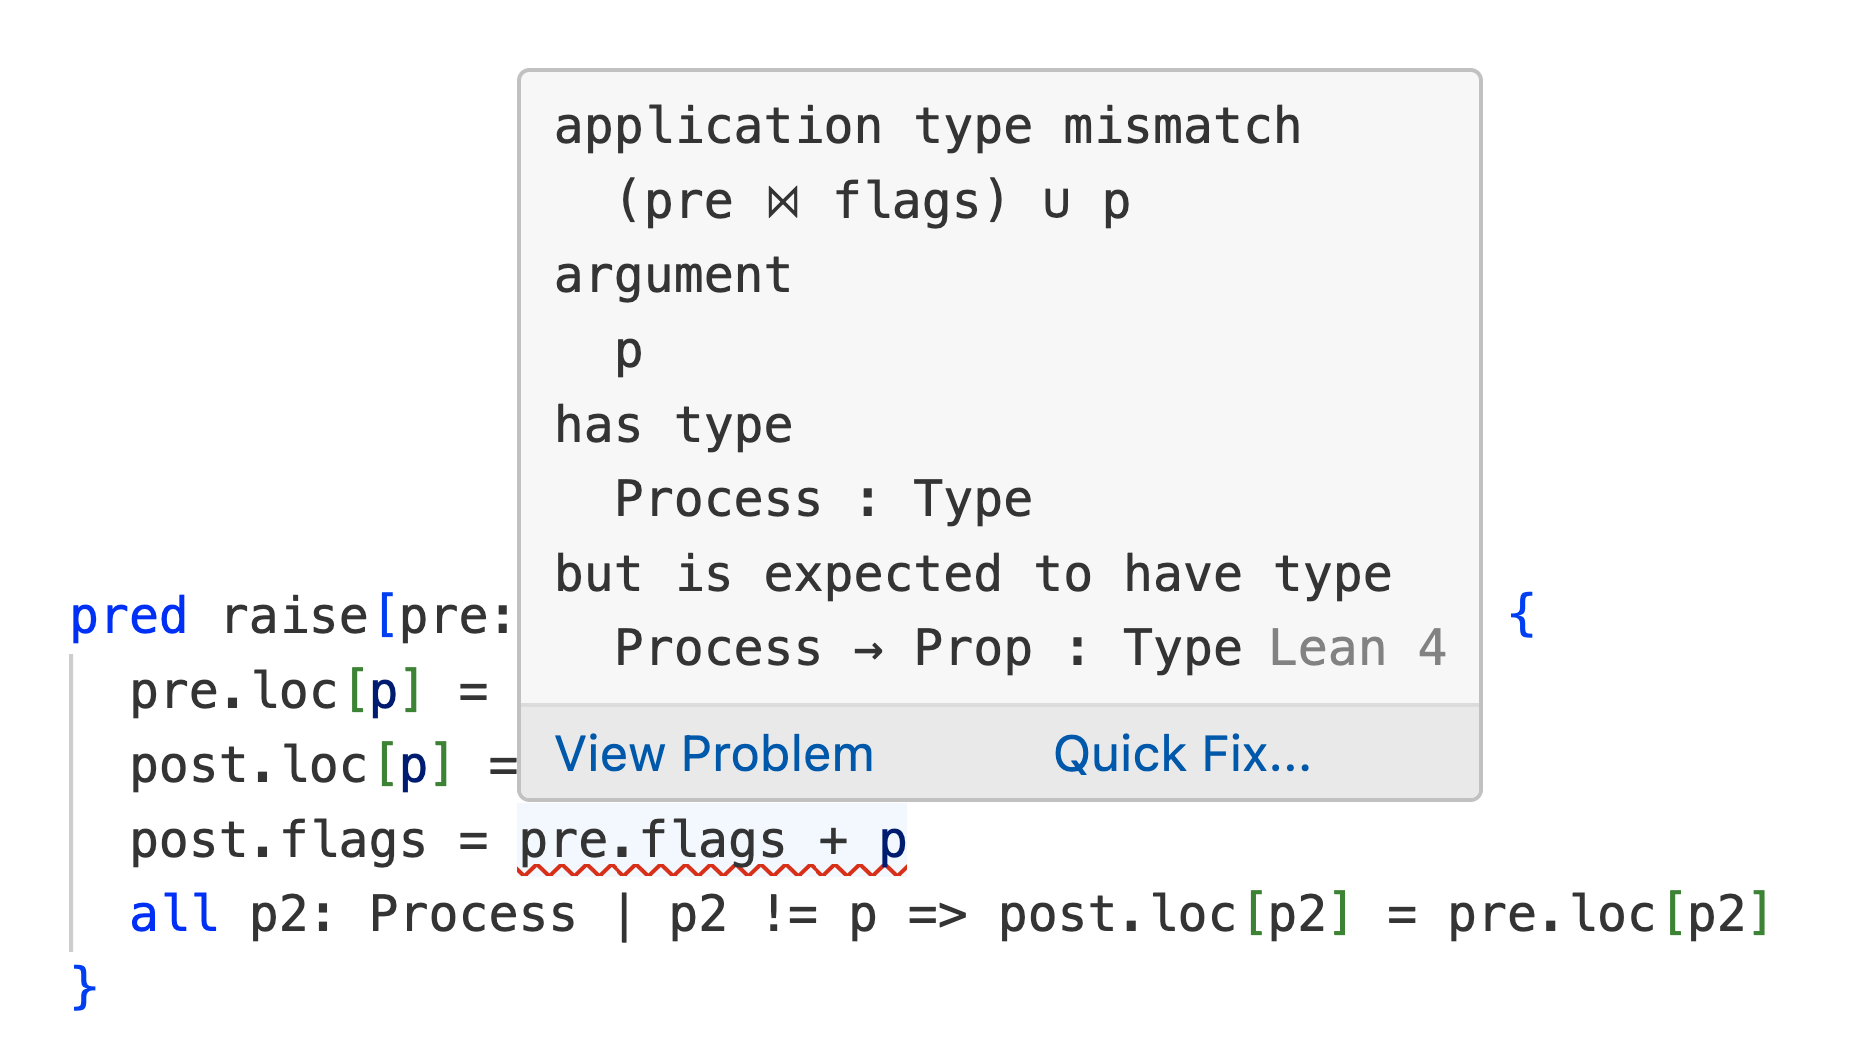
\includegraphics[width=0.5\textwidth,trim={0 0 0 0},clip]{images/screenshots/type-coercion-error.png}}
\end{center}

To solve this, we retrofit syntax onto Forge that allows us to explicitly introduce casts where needed to provide Lean with additional type hints that it can utilize in type unification. We can cast \texttt{p} explicitly, which is a \texttt{Process} type, into a \texttt{Set Process} (the same as \texttt{Process → Prop}) type using the following syntax: 
\begin{forge*}
post.flags = pre.flags - p /* as Set Process */
\end{forge*}
which also coincides with Forge comments to preserve interoperability. 

Future work on the translated type system will involve improving coercions and operations that reduce or completely eliminate the need for explicit type annotations. 

\subsection{Integers}\label{sec:integers}
Forge and Alloy come with a unique integer model---since models are compiled down to boolean constraints to be solved by a SAT solver, integers are severely limited in their bitwidth \cite{jackson2012software,nelson2024artifact}. The default bitwidth on integers in Forge is $4$, which gives us a total of $16$ integers. 

Some programs will inadvertently utilize integer overflow which affects their model in meaningful ways, oftentimes counterintuitively \cite[22]{ngpdbccdlrrvwwk-oopsla-2024}. However, the prevailing documentation on integers in the Forge and Alloy solvers casts this effect as a necessary compromise in the design of the language architecture, and placing a bitwidth on integers is an unavoidable consequence due to the boolean formula-based backend of the language. 

This is an area where Lean shines. Lean has an integer model which is defined using an honest-to-goodness inductive model for the natural numbers \cite{avigad2024theorem}. Lean's integer model is arbitrary precision and designed for proofwriting and numerical reasoning. This includes being able to reason about integers and write functions involving integers that are noncomputable, such as computing the cardinality of a set. 

Here, we depart briefly from the convention that we've been following so far of reproducing Forge as accurately as possible in favor of both more extensive integer support, as well as reduced complexity in implementing integers within our translation. For the most part, we can use Lean's integer and finite set/types libraries out of the box with little modification. 

Our translated Lean models treat all integers as expressions, which makes the translation from an integer expression in Forge to an integer in Lean relatively straightforward. 

Our model is semantically equivalent to running Forge with an arbitrary bitwidth, more than the model would ever exceed and overflow. This gives the most accurate translation of what Forge tries to achieve with integers but is not technically capable of doing. 

Here are two examples adapted from \cite{jackson2012software} that showcase some of the integer features in Forge. 

In Forge, the \texttt{\#} keyword, like on line 4 below, denotes the cardinality of a set. 

\begin{forge}
sig Suit {}
sig Card { suit: one Suit }
pred threeOfAKind[hand: set Card] {
  #hand.suit = 1 and #hand = 3
}
\end{forge}

Fields of sigs can also be integers, and we can do arithmetic on them. By treating all integers as first-class expressions\footnote{Forge denotes integers as atoms or values depending on whether an integer appears in a field or as a result of a computation, but casts seamlessly between \cite{forge-docs,nelson2024artifact}.}, we can also use integers in fields alongside integers that are the result of a set computation. For example, we could define a weighted graph with weighted edges \emph{and} nodes:

\begin{forge}
sig Node {
  node_weight: one Int
}
sig Edge {
  start: one Node,
  end: one Node,
  edge_weight: one Int
}
pred nodeWeightIsEdgeWeightPlusOne[n: Node] {
  n.node_weight = add[1, sum e: { l: Edge | l.start = n } | { e.edge_weight }]
}
\end{forge}

On line 10, we are defining a predicate that states a node $n$'s weight is equal to $1$ plus the sum of edge weights of those edges that start at $n$. 

Of the integer operations, we can easily translate arithmetic operations (addition, subtraction, integer division, remainder, absolute value and sign) as well as inequalities directly into their integer equivalent in Lean. What requires more effort are the notions of counting (cardinality) and quantification in Forge as exemplified above. 

We approach the cardinality problem by using \texttt{Set.ncard}\footnote{More specifically, we do need to utilize the approach in \cref{sec:everything-is-a-set} of using type classes to implement this, since the cardinality of a singleton ought to be $1$. In all other cases, \texttt{Set.ncard} is the implementation of cardinality.}. While this function has a junk value when a set is infinite, we had remedied this earlier in \cref{sec:finiteness} by including \texttt{Fintype} axioms with every Forge type we introduce. Lean knows that every set of a \texttt{Fintype} is a \texttt{Finset} and has an honest-to-goodness cardinality. This allows us to implement sum, max, min, and a summation with a binder (see line 10 of the graph example above) using Lean \texttt{Finset} methods such as \texttt{Finset.sum}, \texttt{Finset.max}, etc. 

To illustrate, the translations of the two predicates (playing card hand and graph) above in Lean, eliding sig and field translations, would be as follows:
\begin{lean*}
def threeOfAKind (hand : Set Card) : Prop :=
  Set.ncard (hand !$\bowtie$! suit) = 1 ∧ Set.ncard hand = 3
\end{lean*}
and 

\begin{lean*}
def nodeWeightIsEdgeWeightPlusOne (n : Node ) : Prop :=
  node_weight n = 1 + Finset.sum { e : Edge | start e = n } edge_weight -- See footnote \footnotemark
\end{lean*}
\footnotetext{There are select details surrounding type coercions, universe levels, and the noncomputability of our integer functions that remain to be resolved. }

While we did need to retrofit additional instance axioms for each type generated to make an integer model work, it is impressive that we were able to extract so much integer functionality out of Forge in within our limited Lean model in the first place. Implementing Forge integers within our translation is also a hallmark of the motivation behind our project in the first place---that in some cases, we can endow \emph{additional} functionality to the Forge specification language by interpreting it in a proof assistant instead of the standard relational Forge implementation. 

The complete translation of Forge integers into Lean is overviewed in \cref{tab:ints} earlier in \cref{sec:forge-model}. 